% 2nd chapter Requirement Analysis
Our clients desired to have a graphic interface like Expresso (working on Caffe framework) for Pytorch.
Their requirement is such an interface that the user can navigate between different tab and each tab correspond to one step of building a neural network so that the user be able to  train and evaluate the imported data.
\section{Functional design}


We decided to create a user friendly application according to the desire of the client so that its easy for them to understand what they are going to do in each tab and we expressed the functional needs accordingly.

\subsection{Data tab} 
    \begin{itemize}
        \item Import Data from the computer (file or directory)that Pytorch can use
        \item Set the import data as Training Data or Test Data
        \item Visualize the Data-parameters (Name, Size, Datasets Mode)
        \item Clear the import data.
    \end{itemize}
    
\subsection{Network tab} 
    \begin{itemize}
        \item Create a network from scratch and edit it.
        \item Load a network from a specific format (json file)  and to visualize it.
        \item Add a Layer from a database (load in background) to the network.
        \item Add an Activation Function from a database (load in background) to the network.
        \item Edit the layer parameter (rename a layer, number edition ...).
        \item Save a network into a specific format(json file).
        \item Choose a Loss Function from a database (load in background) and edit its parameters.
        \item Choose an Optimizer Function from a database (load in background) and edit its parameters.
    \end{itemize}
    
\subsection{Train tab} 
    \begin{itemize}
        \item Choose all Training Parameters (Data to use, Epoch, batchSize).
        \item Visualize Training result (graphics).
        \item Train the network.
    \end{itemize}
    
\subsection{Evaluation tab}
    \begin{itemize}
        \item Choose which data to use for the Evaluation
        \item Choose a Loss Function and its parameters.
        \item Evaluate the current network.
        \item Visualize the network evaluation results.
    \end{itemize}
    
\subsection{Use cases diagrams}
    \subsubsection{PyTorchGUI}
    \begin{figure}[htbp]
        \centering 
        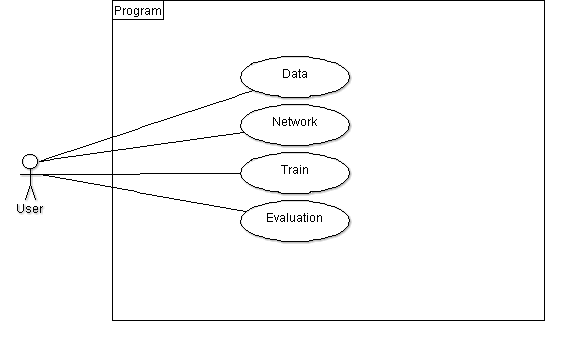
\includegraphics[width=\textwidth]{figures/dcuProgram.png}
        \caption{Use case PyTorchGUI}
    \end{figure}

%stuff to say
There is only one actor that interacts with our application, the user.
There is a lot of use cases in our application, it couldn't be possible to put all of them in only one diagram, thus we designed 5 diagrams, one for each tab and one for the program.
\newline
From everywhere on the application you can switch of tab:
\begin{itemize}
    \item Data
    \item Network
    \item Train
    \item Evaluation
\end{itemize}
%end stuff

\pagebreak

    \subsubsection{Data tab}
    \begin{figure}[htbp]
        \centering 
        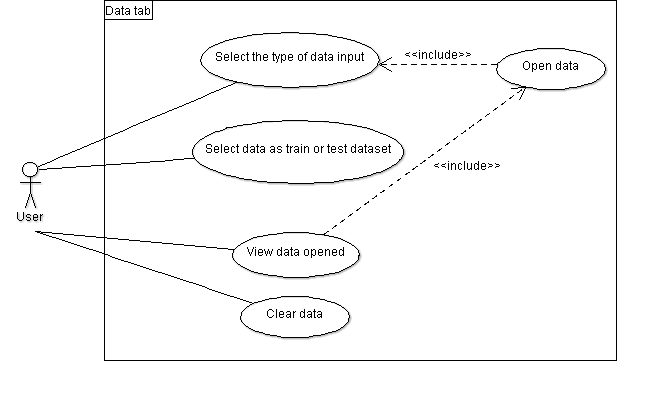
\includegraphics[width=\textwidth]{figures/dcuData.png}
        \caption{Use case Data tab}
    \end{figure}
%stuff to say
%end stuff

\pagebreak

    \subsubsection{Network tab}
    \begin{figure}[htbp]
        \centering 
        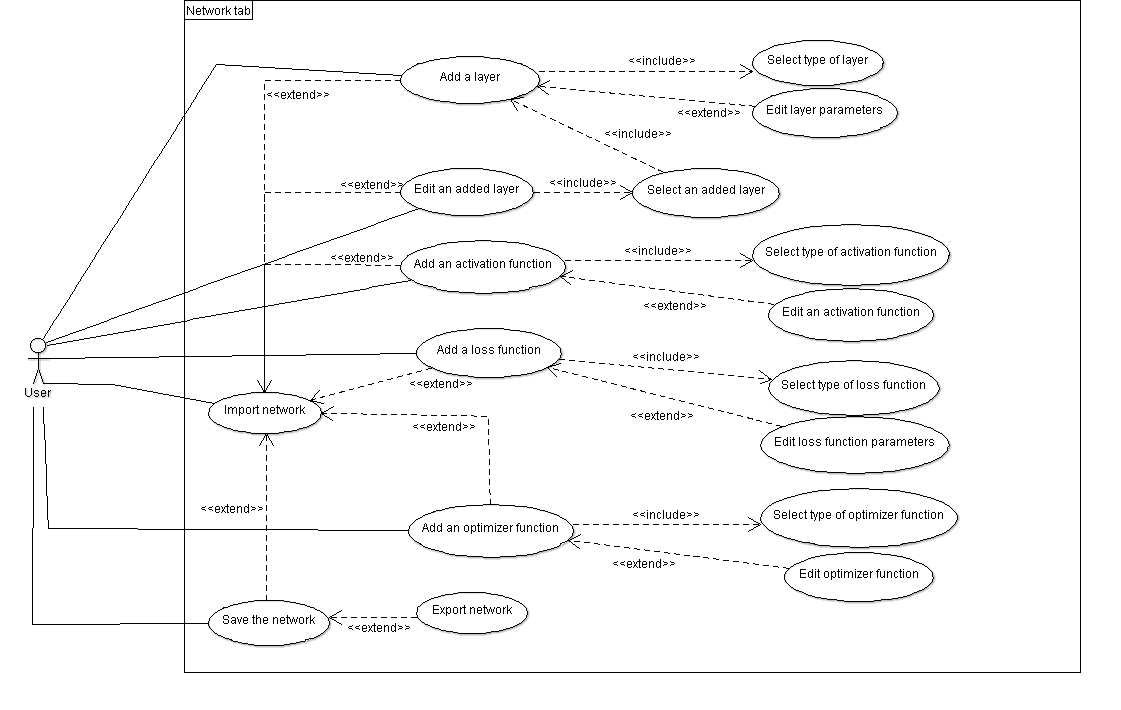
\includegraphics[width=\textwidth]{figures/dcuNetwork.png}
        \caption{Use case Network tab}
    \end{figure}
%stuff to say
%end stuff

\pagebreak
    
    \subsubsection{Train tab}
    \begin{figure}[htbp]
        \centering 
        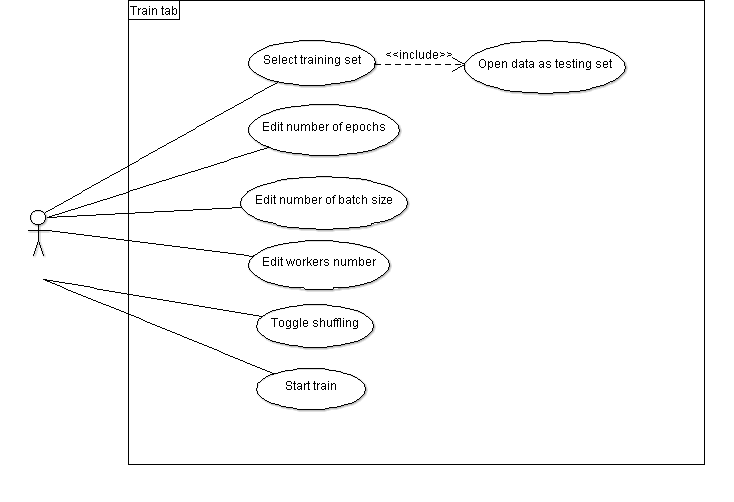
\includegraphics[width=\textwidth]{figures/dcuTrain.png}
        \caption{Use case Train tab}
    \end{figure}
%stuff to say
%end stuff

\pagebreak
    
    \subsubsection{Evaluation tab}
    \begin{figure}[htbp]
        \centering 
        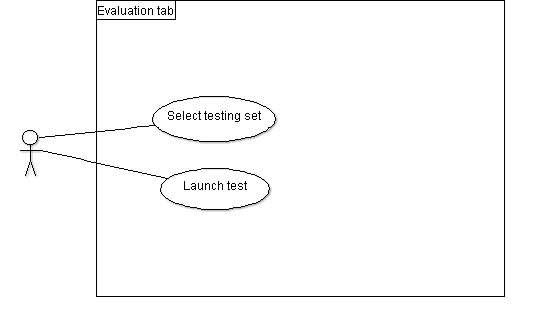
\includegraphics[width=\textwidth]{figures/dcuEvaluation.png}
        \caption{Use case Evaluation tab}
    \end{figure}
%stuff to say
%end stuff
    
\subsection{Scenario}
    Use case: Build a network from scratch, save it, train it, evaluates it
    Actor: User
    Summary: The user wants to create his own network that will operate on data he imported. He wants to save it, train his network on a training dataset he imported too.
    \newline
    
    
    \begin{enumerate}
        \item First the user wants to import his data.
        \item He selects as which type of data he wants his data imported as.
        \item He imports his data by clicking on "Open data".
        \item The application opens an explorer window where he select his data.
        \item Then the data are sent to PyTorch to be transformed to a dataset.
        \item PyTorch returns the dataset to the application.
        \item PyTorchGUI display opened data.
        \item The user switch to the Network tab.
        \item He selects a type of Layer in the dropdown list.
        \item Adds it to the network by clicking on "Add a layer".
        \item The application opens an edition window.
        \item He edits the layer parameters.
        \item Clicks on Add.
        \item Set it as first layer.
        \item Selects a loss function in the dropdown list.
        \item Confirm his choice.
        \item The application opens an edition window.
        \item The user edits the loss function parameters.
        \item Clicks on Set.
        \item Select an optimizer function in the dropdown list.
        \item Confirm his choice.
        \item The application opens an edition window.
        \item The user edits the optimizer function parameters
        \item Save his network
        \item The application opens an explorer window.
        \item The user choose a path.
        \item The application save his network to said path.
        \item The user switch to the Train tab.
        \item He edits the train parameters.
        \item Clicks on "Start Train".
        \item The application build the network from the model the user chose previously.
        \item Then will train the network thanks to PyTorch.
        \item Returns the trained network.
        \item The user switch to the Evaluation tab.
        \item He selects the dataset to evaluate.
        \item Then selects a loss function.
        \item Confirm his choice.
        \item PyTorchGUI opens an edition window.
        \item The user edits loss function parameters.
        \item Adds it to the network.
        \item The application adds the loss function to the network.
        \item The user evaluate the model by clicking on "Launch test".
        \item PyTorchGUI evaluate the dataset with created network thanks to PyTorch.
        \item The application returns the neural network.
        \item Then displays it.
        \item The user can see his neural network he created, trained and evaluated.
    \end{enumerate}
        
    
    
    \subsubsection{Sequence diagram}
    \begin{figure}[htbp]
        \vspace*{-1.5cm}
        \centerline{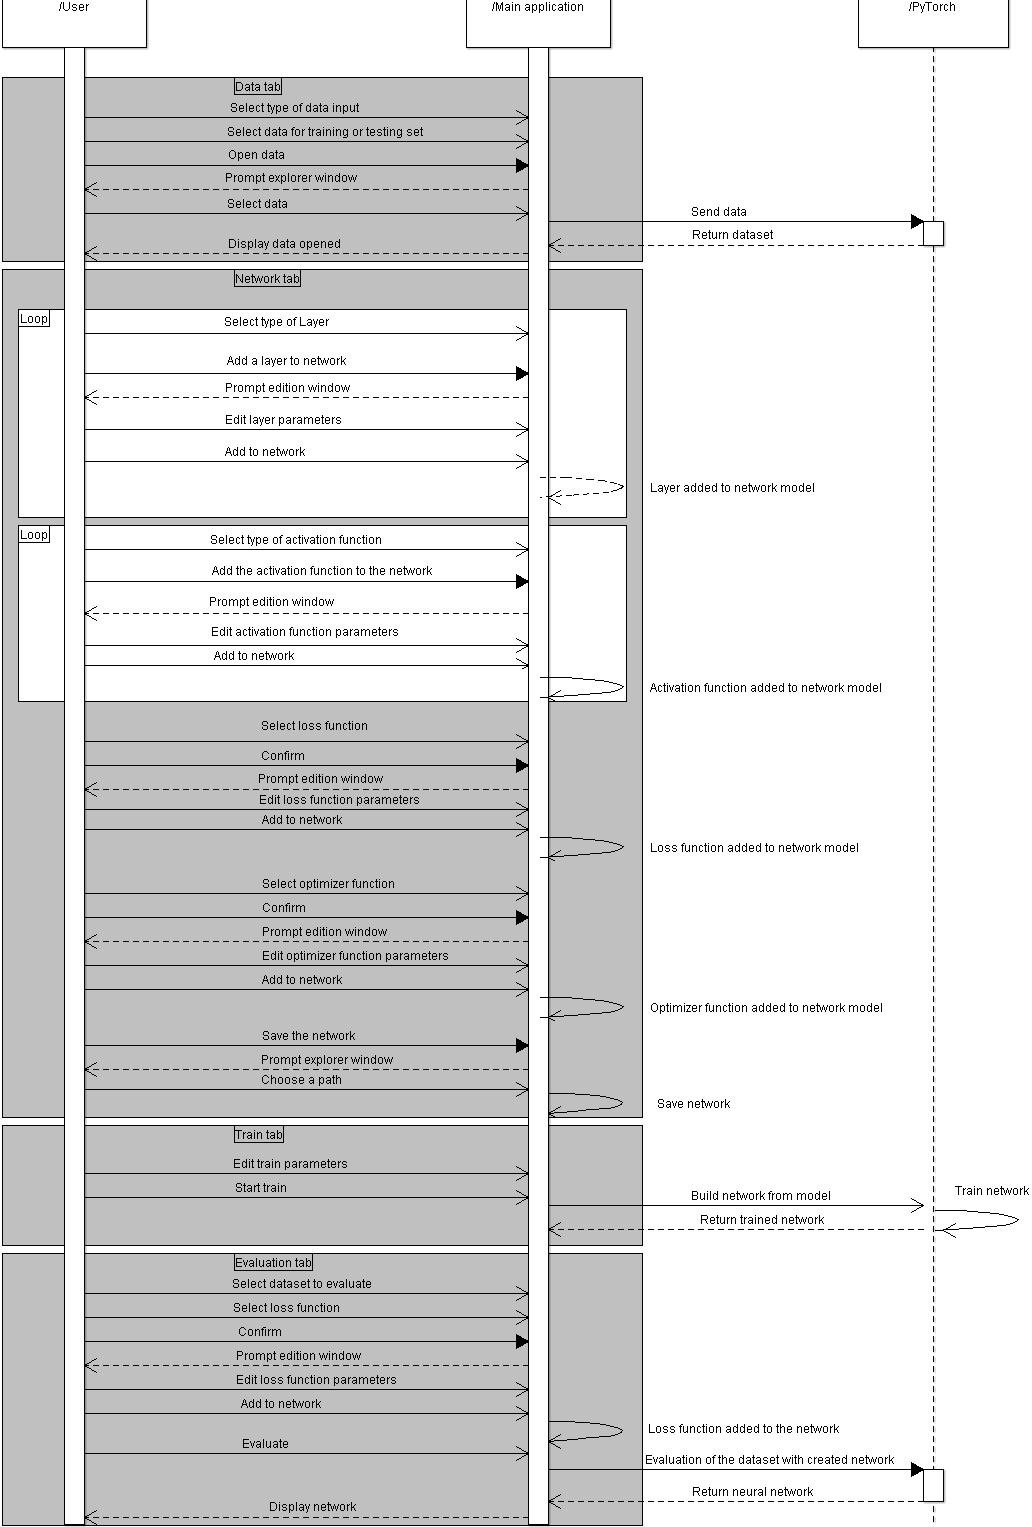
\includegraphics[scale=0.65]{figures/diagSeq.png}}
        \caption{Sequence diagram of building network from scratch}
    \end{figure}
\newpage

\subsection{Constraints}

\begin{itemize}
\item Platform-compatibility : The app has to be compatible with Linux. If possible, we will try to make it work also with other platforms.
\item Maintainability : We have to develop our application in a way that allows future developers to extend the functionalities. Also, we have to make sure that our app will easily be compatible with future versions of PyTorch.
\end{itemize}

\subsection{Choice of application type}

To develop our application we were thinking about two types of applications. These two choices are a Web-Service, or a regular application.
In order to choose which type of application to develop we drew up a table of advantages and disadvantages.

\begin{itemize}
    \item Web-Service advantages :
    \begin{itemize}
         \item The Web application can be used by all users anywhere and when they want if they are connected to Internet. Furthermore, this facilitates a simple to get a multi-platform application.
        \item The application is always up to date, if it needs an update we only have to update the server whereas a simple application have to be updated on all users' computer. The app is more flexible.
        \item The deployment of the app is easier
        \item It could facilitate the extension of the app to add features
    \end{itemize}
\end{itemize}

 
 \begin{itemize}
    \item Web-Service drawbacks :
    \begin{itemize}
         \item Users need to be connected and to have good network performance (fast and stable) especially in case of big data exchanges. In addition, the server could have to support many users at the same time. Even if the app is running in local, they need to have a good central server, which needs a more complex architecture.
        \item With the same hardware, performances are lower than a native application, we have to exchange data with the server so it must take a long time before getting results especially if we have a lot of data in addition of the time of calculation.
        \item Complex visual effects like drawing a graph could be more complicated to implement
        
    \end{itemize}
\end{itemize}

  \begin{itemize}
    \item Native Application advantages :
    \begin{itemize}
        \item Users don't need an Internet connection.
        \item It has got better performances, better time of calculation, better time of response.(Faster than a Web-Service)
    \end{itemize}
\end{itemize}
\begin{itemize}
    \item Native Application disadvantages :
    \begin{itemize}
        \item Every user have to install the application on his personal computer.
         \item If the application needs an update, we have to upgrade all the computers equipped with the application.
    \end{itemize}
\end{itemize}

\textbf{Our choice :}
Since both options seemed quite equivalent for us, and since having a web-service deployment wasn't a need for the project, we decided to go on to the \textbf{Native Application}. Indeed, this will perfectly allow us to implement all needed features with performance similar to those of PyTorch by itself.


\pagebreak
